% \documentclass{article}
% \usepackage{tikz}
% \usetikzlibrary{patterns, decorations.pathmorphing, arrows.meta}
% \newcommand{\pyvar}[1]{\texttt{#1}}
% \usepackage{graphicx,scalerel}
% \usepackage{adjustbox}
% \usetikzlibrary{calc}
% % H (red)
\newcommand{\ThH}{\textcolor{red}{3\heartsuit}}  
\newcommand{\TwH}{\textcolor{red}{2\heartsuit}}  
\newcommand{\FoH}{\textcolor{red}{4\heartsuit}}   
\newcommand{\FiH}{\textcolor{red}{5\heartsuit}}   
\newcommand{\SiH}{\textcolor{red}{6\heartsuit}}    
\newcommand{\SeH}{\textcolor{red}{7\heartsuit}}  
\newcommand{\EH}{\textcolor{red}{8\heartsuit}}  
\newcommand{\NH}{\textcolor{red}{9\heartsuit}}   
\newcommand{\TeH}{\textcolor{red}{10\heartsuit}}   
\newcommand{\JH}{\textcolor{red}{J\heartsuit}}    
\newcommand{\QH}{\textcolor{red}{Q\heartsuit}}   
\newcommand{\KH}{\textcolor{red}{K\heartsuit}}    
\newcommand{\AH}{\textcolor{red}{A\heartsuit}}     

% D (red)
\newcommand{\ThD}{\textcolor{red}{3\diamondsuit}}  
\newcommand{\TwD}{\textcolor{red}{2\diamondsuit}}  
\newcommand{\FoD}{\textcolor{red}{4\diamondsuit}}   
\newcommand{\FiD}{\textcolor{red}{5\diamondsuit}}   
\newcommand{\SiD}{\textcolor{red}{6\diamondsuit}}    
\newcommand{\SeD}{\textcolor{red}{7\diamondsuit}}  
\newcommand{\ED}{\textcolor{red}{8\diamondsuit}}  
\newcommand{\ND}{\textcolor{red}{9\diamondsuit}}   
\newcommand{\TeD}{\textcolor{red}{10\diamondsuit}}   
\newcommand{\JD}{\textcolor{red}{J\diamondsuit}}    
\newcommand{\QD}{\textcolor{red}{Q\diamondsuit}}   
\newcommand{\KD}{\textcolor{red}{K\diamondsuit}}    
\newcommand{\AD}{\textcolor{red}{A\diamondsuit}}     

% C (black)
\newcommand{\ThC}{\textcolor{black}{3\clubsuit}}   
\newcommand{\TwC}{\textcolor{black}{2\clubsuit}}   
\newcommand{\FoC}{\textcolor{black}{4\clubsuit}}    
\newcommand{\FiC}{\textcolor{black}{5\clubsuit}}    
\newcommand{\SiC}{\textcolor{black}{6\clubsuit}}     
\newcommand{\SeC}{\textcolor{black}{7\clubsuit}}   
\newcommand{\EC}{\textcolor{black}{8\clubsuit}}   
\newcommand{\NC}{\textcolor{black}{9\clubsuit}}    
\newcommand{\TeC}{\textcolor{black}{10\clubsuit}}    
\newcommand{\JC}{\textcolor{black}{J\clubsuit}}    
\newcommand{\QC}{\textcolor{black}{Q\clubsuit}}   
\newcommand{\KC}{\textcolor{black}{K\clubsuit}}    
\newcommand{\AC}{\textcolor{black}{A\clubsuit}}     

% S (black)
\newcommand{\ThS}{\textcolor{black}{3\spadesuit}}   
\newcommand{\TwS}{\textcolor{black}{2\spadesuit}}   
\newcommand{\FoS}{\textcolor{black}{4\spadesuit}}    
\newcommand{\FiS}{\textcolor{black}{5\spadesuit}}    
\newcommand{\SiS}{\textcolor{black}{6\spadesuit}}     
\newcommand{\SeS}{\textcolor{black}{7\spadesuit}}   
\newcommand{\ES}{\textcolor{black}{8\spadesuit}}   
\newcommand{\NS}{\textcolor{black}{9\spadesuit}}    
\newcommand{\TeS}{\textcolor{black}{10\spadesuit}}    
\newcommand{\JS}{\textcolor{black}{J\spadesuit}}    
\newcommand{\QS}{\textcolor{black}{Q\spadesuit}}   
\newcommand{\KS}{\textcolor{black}{K\spadesuit}}    
\newcommand{\AS}{\textcolor{black}{A\spadesuit}}     

% \begin{document}
% SUITS = ['♣', '♦', '♥', '♠'] 


\begin{figure}[h]
    \centering
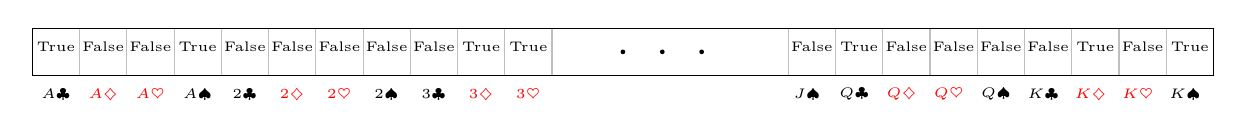
\begin{tikzpicture}
    % Define grid dimensions
    \def\n{1} % N = 5 rows
    \def\m{25} % M = 5 columns
    \def\cellsize{0.6} % Size of each cell

    % Draw the grid
    \foreach \i in {0,...,\n} {
        \draw[lightgray] (0,\i*\cellsize) -- (\m*\cellsize,\i*\cellsize); % Horizontal lines
    }
    % \foreach \j in {0,...,\m} {
    %     \draw[lightgray] (\j*\cellsize,0) -- (\j*\cellsize,\n*\cellsize); % Vertical lines
    % }

    % Place dots in the middle row (row 3, columns 2, 3, and 4)
    \foreach \j in {0,1,2} {
        \fill[black] ({(1-\j)/2+\m*\cellsize/2+0.5}, 0.5*\cellsize) circle (0.03); % Dots
    }

    \foreach \j in {0,...,\m} {
        \ifnum\j<12 % Check if j < 10
            \draw[lightgray] (\j*\cellsize,0) -- (\j*\cellsize,\n*\cellsize); % Draw line
        \else
            \ifnum\j>15 % Check if j > 20
                \draw[lightgray] (\j*\cellsize,0) -- (\j*\cellsize,\n*\cellsize); % Draw line
            \fi
        \fi
        }

    % Draw the outer rectangle
    \draw[black] (0,0) rectangle (\m*\cellsize, \n*\cellsize);

    % Add the shape label below the grid
    % \node[below] at ({\m/2*\cellsize}, 4.5*\cellsize) {\pyvar{t\_z[:,0,:]}};

    % \draw[->, thin, decorate, decoration={coil, segment length=7mm, amplitude=2mm}] 
    %     ({(\m-2)*\cellsize+0.1}, \n*\cellsize+0.1) -- ++(2,1) % Arrow starts at (5,5) and extends 2 units right
    %     node[above, right, align=left] {\small A card has \\ \;$\cdot$ a rank\\ \;$\cdot$ a suit}; % Text at the end of the arrow

    \node at (0.5*\cellsize, \n*\cellsize-0.4*\cellsize) {\tiny \py{True}};
    \node at (1.5*\cellsize, \n*\cellsize-0.4*\cellsize) {\tiny \py{False}};
    \node at (2.5*\cellsize, \n*\cellsize-0.4*\cellsize) {\tiny \py{False}};
    \node at (3.5*\cellsize, \n*\cellsize-0.4*\cellsize) {\tiny \py{True}};
    \node at (4.5*\cellsize, \n*\cellsize-0.4*\cellsize) {\tiny \py{False}};
    \node at (5.5*\cellsize, \n*\cellsize-0.4*\cellsize) {\tiny \py{False}};
    \node at (6.5*\cellsize, \n*\cellsize-0.4*\cellsize) {\tiny \py{False}};
    \node at (7.5*\cellsize, \n*\cellsize-0.4*\cellsize) {\tiny \py{False}};
    \node at (8.5*\cellsize, \n*\cellsize-0.4*\cellsize) {\tiny \py{False}};
    \node at (9.5*\cellsize, \n*\cellsize-0.4*\cellsize) {\tiny \py{True}};
    \node at (10.5*\cellsize, \n*\cellsize-0.4*\cellsize) {\tiny\py{True}};
    
    \node at (0.5*\cellsize, \n*\cellsize-1.4*\cellsize) {\tiny $\AC$};
    \node at (1.5*\cellsize, \n*\cellsize-1.4*\cellsize) {\tiny $\AD$};
    \node at (2.5*\cellsize, \n*\cellsize-1.4*\cellsize) {\tiny $\AH$};
    \node at (3.5*\cellsize, \n*\cellsize-1.4*\cellsize) {\tiny $\AS$};
    \node at (4.5*\cellsize, \n*\cellsize-1.4*\cellsize) {\tiny $\TwC$};
    \node at (5.5*\cellsize, \n*\cellsize-1.4*\cellsize) {\tiny $\TwD$};
    \node at (6.5*\cellsize, \n*\cellsize-1.4*\cellsize) {\tiny $\TwH$};
    \node at (7.5*\cellsize, \n*\cellsize-1.4*\cellsize) {\tiny $\TwS$};
    \node at (8.5*\cellsize, \n*\cellsize-1.4*\cellsize) {\tiny $\ThC$};
    \node at (9.5*\cellsize, \n*\cellsize-1.4*\cellsize) {\tiny $\ThD$};
    \node at (10.5*\cellsize,\n*\cellsize-1.4*\cellsize) {\tiny $\ThH$};

    \node at (16.5*\cellsize, \n*\cellsize-0.4*\cellsize) {\tiny \py{False}};
    \node at (17.5*\cellsize, \n*\cellsize-0.4*\cellsize) {\tiny \py{True}};
    \node at (18.5*\cellsize, \n*\cellsize-0.4*\cellsize) {\tiny \py{False}};
    \node at (19.5*\cellsize, \n*\cellsize-0.4*\cellsize) {\tiny \py{False}};
    \node at (20.5*\cellsize, \n*\cellsize-0.4*\cellsize) {\tiny \py{False}};
    \node at (21.5*\cellsize, \n*\cellsize-0.4*\cellsize) {\tiny \py{False}};
    \node at (22.5*\cellsize, \n*\cellsize-0.4*\cellsize) {\tiny \py{True}};
    \node at (23.5*\cellsize, \n*\cellsize-0.4*\cellsize) {\tiny \py{False}};
    \node at (24.5*\cellsize, \n*\cellsize-0.4*\cellsize) {\tiny \py{True}};
    
    \node at (16.4*\cellsize, \n*\cellsize-1.4*\cellsize) {\tiny $\JS$};
    \node at (17.4*\cellsize, \n*\cellsize-1.4*\cellsize) {\tiny $\QC$};
    \node at (18.4*\cellsize, \n*\cellsize-1.4*\cellsize) {\tiny $\QD$};
    \node at (19.4*\cellsize, \n*\cellsize-1.4*\cellsize) {\tiny $\QH$};
    \node at (20.4*\cellsize, \n*\cellsize-1.4*\cellsize) {\tiny $\QS$};
    \node at (21.4*\cellsize, \n*\cellsize-1.4*\cellsize) {\tiny $\KC$};
    \node at (22.4*\cellsize, \n*\cellsize-1.4*\cellsize) {\tiny $\KD$};
    \node at (23.4*\cellsize, \n*\cellsize-1.4*\cellsize) {\tiny $\KH$};
    \node at (24.4*\cellsize, \n*\cellsize-1.4*\cellsize) {\tiny $\KS$};

    
\end{tikzpicture}
\caption{\py{t\_inp} tensor at the beginning of the game for the initial setup shown in Table~\ref{table:deck9}}
\label{fig:deck}
\end{figure}
% \end{document}
% alex: 4♣ 4♢ 7♢ Q♣ 
% bob: 3♢ 3♡ 5♣ K♠ 
% Pool: A♣ A♠ 9♢ K♢
